
    \chapter{Estudo de caso e avaliação do modelo}
    Para validar o modelo de segurança proposto, utilizamos a aplicação ``Herd Financial'' do projeto GoatDroid para demonstração dos casos de uso dos requisitos de segurança modelados. Além disso, avaliamos a conformidade e garantia do modelo por meio da adequação à certificação de segurança PCI DSS.

    \section{Estudo de caso}
    Para avaliar a eficácia e viabilidade dos requisitos de segurança modelados por meio da demonstração dos casos de uso, adotamos uma abordagem estruturada dividida em duas etapas principais. Primeiro, identificamos e analisamos algumas das fragilidades presentes na aplicação Herd Financial, utilizando como referência o \citeonline{herd2016}, e logo após apontamos os requisitos de segurança modelados na etapa anterior capazes de mitigar essas vulnerabilidades, demonstrando exemplos de código em Java.


    \subsection{Visão Geral do Herd Financial}
    
    Herd Financial é uma aplicação bancária fictícia projetada pela \citeonline{goat2024} como parte do projeto GoatDroid, uma plataforma de teste para identificar e explorar vulnerabilidades em aplicações Android. O objetivo principal do Herd Financial é simular um ambiente de aplicação bancária real, permitindo que desenvolvedores e pesquisadores de segurança testem e compreendam as falhas comuns encontradas em aplicativos bancários móveis. A aplicação oferece funcionalidades típicas de um aplicativo bancário, como:

    \begin{itemize}[topsep=3pt, partopsep=3pt, itemsep=3pt, parsep=3pt]
        \item Visualização de Saldo: Os usuários podem verificar o saldo de suas contas bancárias.
        \item Transferência de Fundos: Permite a transferência de dinheiro entre contas.
        \item Gerenciamento de Contas: Inclui funcionalidades para adicionar, editar e remover contas bancárias.
        \item Histórico de Transações: Exibe um registro das transações realizadas pelo usuário.
    \end{itemize}

    Essas funcionalidades, enquanto fornecem um cenário realista para os usuários, também incorporam várias vulnerabilidades propositais. A presença dessas falhas intencionais faz do Herd Financial uma ferramenta valiosa para testar as práticas de segurança recomendadas e avaliar a eficácia das estratégias de mitigação.

    Através da análise do Herd Financial, podemos aplicar o modelo de segurança proposto e observar como ele se comporta em um ambiente de teste controlado. Isso nos permite identificar áreas de melhoria e validar a eficácia das medidas de segurança implementadas, oferecendo insights práticos que podem ser aplicados em desenvolvimentos futuros de aplicações bancárias reais.

    \subsection{Requisitos de autenticação e autorização}
    Herd Financial inicialmente utilizava um sistema básico de autenticação com senha mostrado na figura \ref{login}, sem suporte a autenticação multifatorial (MFA).

    \begin{figure}[H]
    \centering 
    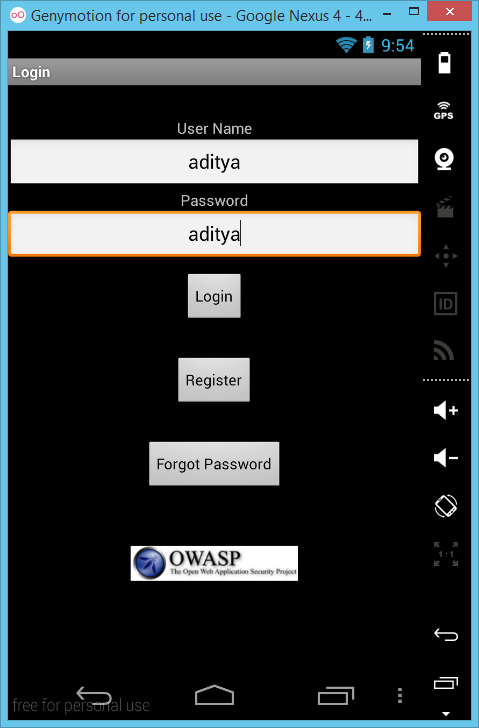
\includegraphics[width=7cm]{Imagens/loginherd.png} 
    \caption{Login de usuário do Herd Financial}
    Fonte: \citeonline{herd2016}
    \label{login}
    
    \end{figure}

    Este método simples de autenticação deixava a aplicação vulnerável a ataques de força bruta e acessos não autorizados. O modelo recomenda a autenticação multifatorial, adicionando uma camada adicional de segurança ao exigir um segundo fator de autenticação. No caso, um algoritmo TOTP.

    O código apresentado mostra como utilizar o Firebase para implementar o TOTP, onde um código temporário gerado por um aplicativo autenticador é requerido além da senha tradicional. Isso adiciona uma camada adicional de segurança, dificultando o acesso não autorizado mesmo que a senha do usuário seja comprometida.
    \\

    \begin{scriptsize}
    \estiloJava
    \begin{lstlisting}[caption={Autenticação por TOTP Utilizando Firebase}, label=lst:javacode]
    when (exception.resolver.hints[selectedIndex].factorId) {
        TotpMultiFactorGenerator.FACTOR_ID -> {
            val otpFromAuthenticator = // OTP escrito pelo usuário.
            val assertion = TotpMultiFactorGenerator.getAssertionForSignIn(
                exception.resolver.hints[selectedIndex].uid,
                otpFromAuthenticator
            )
            exception.resolver.resolveSignIn(assertion)
                .addOnSuccessListener { result ->
                    // Successfully signed in!
                    Log.d(TAG, "signInWithTOTP:success");
                }
                .addOnFailureListener { resolveError ->
                    Toast.makeText(TOTPActivity.this, "Invalid or expired OTP.",
                                Toast.LENGTH_SHORT).show();
                }
        }
    }
    \end{lstlisting}
    \end{scriptsize}

    Na maioria das vezes, após a autenticação em um aplicativo Android, o usuário é enviado para uma nova atividade com as funcionalidades da aplicação. Manter essas atividades exportadas e até mesmo sem permissões personalizadas, deixam a aplicação suscetível ao acesso não autorizado. 
    
    No aplicativo HerdFinancial, a atividade org.owasp.goatdroid.herdfinancial.activities.Main foi exportada e também não tem nenhuma permissão personalizada. O que permite a um malware simplesmente passar uma intenção e iniciar a atividade específica, como mostrado na figura \ref{drozer}.

    \begin{figure}[H]
    \centering 
    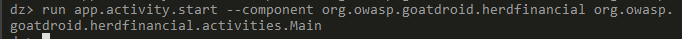
\includegraphics[width=16cm]{Imagens/drozer.png} 
    \caption{Acesso não autorizado utilizando Drozer}
    Fonte: \citeonline{herd2016}
    \label{drozer}
    \end{figure}

    Depois disso, o Herd Financial é iniciado com a conta padrão e podem ser feito coisas como transferir o dinheiro para a conta de outra pessoa, como vemos na figura \ref{main}. 

    \begin{figure}[H]
    \centering 
    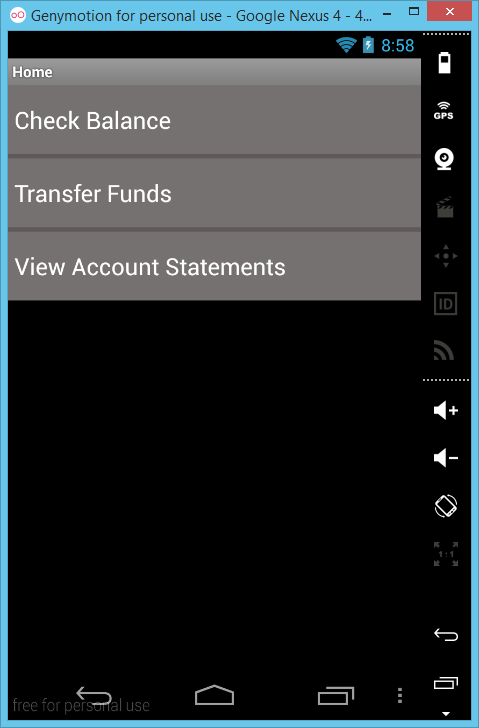
\includegraphics[width=6cm]{Imagens/acmain.png} 
    \caption{Tela inicial}
    Fonte: \citeonline{herd2016}
    \label{main}
    \end{figure}

    Ao utilizar as configurações corretas e permissões nos componente do android, bloqueamos esse tipo de interação. O modelo propõe uso de componentes exportados apenas quando necessário. 

    O código apresentado exemplifica como configurar componentes do Android para não serem exportados (android:exported="false"), garantindo que apenas o próprio aplicativo possa iniciar essas atividades. Ao limitar a exportação de componentes, o modelo previne que aplicativos externos interajam de forma indesejada com o aplicativo, aumentando a segurança contra acessos não autorizados.
    \\

    \begin{scriptsize}
    \estiloJava
    \begin{lstlisting}[caption={Componentes exportados}, label=lst:javacode]
    <activity android:name=".SensiveActivity" android:exported="false" >
        <intent-filter>
            <action android:name="EXAMPLE_ACTIVITY" />
            <category android:name="android.intent.category.LAUNCHER" />
        </intent-filter>
    </activity>

    <service
        android:name=".MessagingService"
        android:exported="false">
        <intent-filter>
            <action android:name="com.google.firebase.MESSAGING_EVENT" />
        </intent-filter>
    </service>

    <receiver android:name=".SensiveReceiver" android:exported="false">
        <intent-filter>
            <action android:name="EXAMPLE_BROADCAST" />
        </intent-filter>
    </receiver>
    
    \end{lstlisting}
    \end{scriptsize}


    Caso seja necessário a exportação, é fundamental definir permissões de segurança apropriadas e validar informações recebidas para componentes sensíveis. 

    O código demonstra como aplicar permissões de segurança apropriadas e filtrar intenções recebidas, garantindo que apenas aplicativos autorizados possam interagir com componentes sensíveis. Essa prática previne que dados sejam acessados ou manipulados por aplicativos não confiáveis, mitigando vulnerabilidades como ataques de malwares à aplicação.
    \\

    \begin{scriptsize}
    \estiloJava
    \begin{lstlisting}[caption={Permissões no Android e filtro de intenção}, label=lst:javacode]
    // Permissões
    <permission android:name="com.example.myapp.MY_PERMISSION" android:protectionLevel="signature" />
    
    <provider
        android:name=".MyContentProvider"
        android:authorities="com.example.myapp.provider"
        android:exported="true"
        android:permission="android.permission.READ_PROVIDER"
    </provider>


    // Verificação de intenção
    Intent intent = getIntent()
    Intent forward = (Intent) intent.getParcelableExtra("key");
    ComponentName name = forward.resolveActivity(getPackageManager());
    if (name.getPackageName().equals("safe_package") &&
            name.getClassName().equals("safe_class")) {
        startActivity(forward);
    }

    // Sanitização de intenção
    Intent intent = new  IntentSanitizer.Builder()
     .allowComponent("com.example.ActivityA")
     .allowData("com.example")
     .allowType("text/plain")
     .build()
     .sanitizeByThrowing(intent);
        
    \end{lstlisting}
    \end{scriptsize}

    Outra proteção recomendada para esses casos é o uso de Pin ou biometria para validar as ações do usuário. Assim garantindo que mesmo em contas comprometidas não seja possível realizar ações maliciosas.

    O código fornecido implementa autenticação biométrica em Android, garantindo que transações e pagamentos, só possam ser realizadas após a validação da identidade do usuário através de biometria. Isso adiciona uma camada extra de segurança, protegendo as ações do usuário contra acessos não autorizados, mesmo em casos onde a senha tenha sido comprometida.
    \\

    \begin{scriptsize}
    \estiloJava
    \begin{lstlisting}[caption={Autenticação por digital}, label=lst:javacode]
    private Executor executor;
    private BiometricPrompt biometricPrompt;
    private BiometricPrompt.PromptInfo promptInfo;
    
    @Override
    protected void onCreate(Bundle savedInstanceState) {
        super.onCreate(savedInstanceState);
        setContentView(R.layout.activity_login);
        executor = ContextCompat.getMainExecutor(this);
        biometricPrompt = new BiometricPrompt(MainActivity.this,
                executor, new BiometricPrompt.AuthenticationCallback() {
            @Override
            public void onAuthenticationError(int errorCode,
                    @NonNull CharSequence errString) {
                super.onAuthenticationError(errorCode, errString);
                Toast.makeText(getApplicationContext(),
                    "Authentication error: " + errString, Toast.LENGTH_SHORT)
                    .show();
            }
    
            @Override
            public void onAuthenticationSucceeded(
                    @NonNull BiometricPrompt.AuthenticationResult result) {
                super.onAuthenticationSucceeded(result);
                Toast.makeText(getApplicationContext(),
                    "Authentication succeeded!", Toast.LENGTH_SHORT).show();
            }
    
            @Override
            public void onAuthenticationFailed() {
                super.onAuthenticationFailed();
                Toast.makeText(getApplicationContext(), "Authentication failed",
                    Toast.LENGTH_SHORT)
                    .show();
            }
        });
    
        promptInfo = new BiometricPrompt.PromptInfo.Builder()
                .setTitle("Biometric login for my app")
                .setSubtitle("Log in using your biometric credential")
                .setNegativeButtonText("Use account password")
                .build();
    

        Button biometricLoginButton = findViewById(R.id.biometric_login);
        biometricLoginButton.setOnClickListener(view -> {
                biometricPrompt.authenticate(promptInfo);
        });
    }
    \end{lstlisting}
    \end{scriptsize}
    

    \subsection{Requisitos de confidencialidade e integridade}

    Outro ponto importante são as informações armazenadas pela aplicação. Como podemos ver na figura \ref{chave}, o Herd Financial armazena chaves sensíveis no código fonte do aplicativo. Dessa forma, qualquer um com o arquivo da aplicação pode obter a senha usando engenharia reversa.

    \begin{figure}[H]
    \centering 
    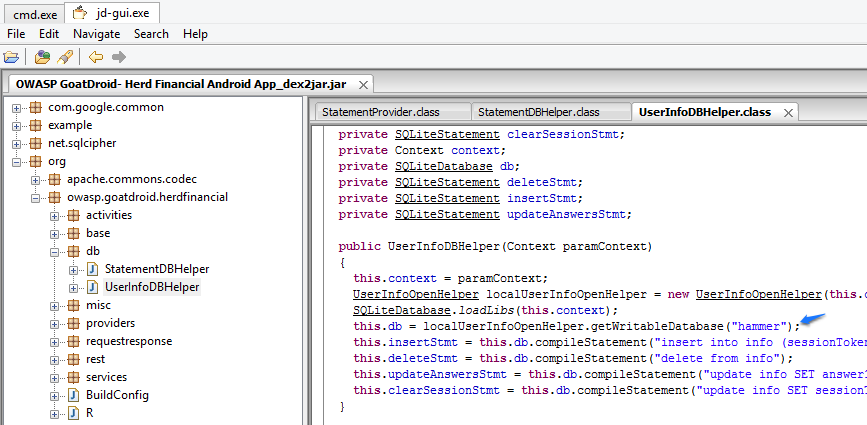
\includegraphics[width=14cm]{Imagens/hammer.png} 
    \caption{Informação vazada no código fonte}
    Fonte: \citeonline{herd2016}
    \label{chave}
    \end{figure}

    Além disso, a aplicação também guarda credenciais no armazenamento interno do dispositivo, como podemos ver nas imagens \ref{internal}, o que torna possível aos usuários maliciosos visualizar e utilizar essas informações. 
    
    \begin{figure}[H]
    \centering 
    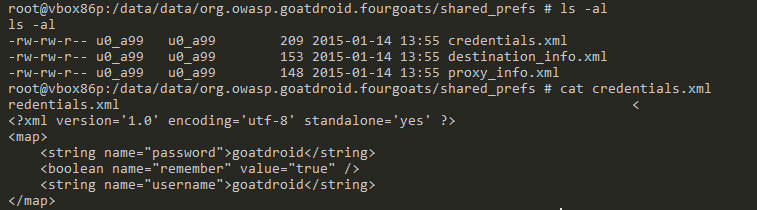
\includegraphics[width=15cm]{Imagens/internal.png} 
    \caption{Informação salva no armazenamento interno}
    Fonte: \citeonline{herd2016}
    \label{internal}
    \end{figure}


    Desse modo, o modelo proposto recomenda o uso de métodos de criptografia para o armazenamento de chaves e senhas. O uso de criptografia forte não só dificulta o acesso não autorizado, mas também garante a confidencialidade das informações, mesmo em caso de comprometimento de outros mecanismos de segurança.

    O código apresentado utiliza criptografia AES com chave de 256 bits e modo de operação CBC ou SHA-256 para proteger dados sensíveis armazenados localmente. A criptografia assegura que, mesmo se um atacante acessar o armazenamento, os dados permanecerão ininteligíveis sem a chave de decriptação correta, garantindo a confidencialidade das informações armazenadas.
    \\

    \begin{scriptsize}
    \estiloJava
    \begin{lstlisting}[caption={Uso de criptografia para armazenamento de dados}, label=lst:javacode]
    // Criptografia assimétrica utilizando o algoritmo AES
    byte[] plaintext = "Texto plano";
    KeyGenerator keygen = KeyGenerator.getInstance("AES");
    keygen.init(256);
    SecretKey key = keygen.generateKey();
    Cipher cipher = Cipher.getInstance("AES/CBC/PKCS5PADDING");
    cipher.init(Cipher.ENCRYPT_MODE, key);
    byte[] ciphertext = cipher.doFinal(plaintext);
    byte[] iv = cipher.getIV();


    // Criptografia de Hash utilizando o algoritmo SHA-256
    byte[] message = "Texto plano";
    MessageDigest md = MessageDigest.getInstance("SHA-256");
    byte[] digest = md.digest(message);
    
    \end{lstlisting}
    \end{scriptsize}

    Seguindo a mesma lógica, a aplicação também tem fragilidades encontradas nos dados em transito. O uso de métodos de criptografia fracos e a falta de verificações de certificados digitais permite que atacantes realizem ataques man-in-the-middle, interceptando e manipulando a comunicação entre o aplicativo e o servidor, como vemos na figura \ref{burp}. 

    \begin{figure}[H]
    \centering 
    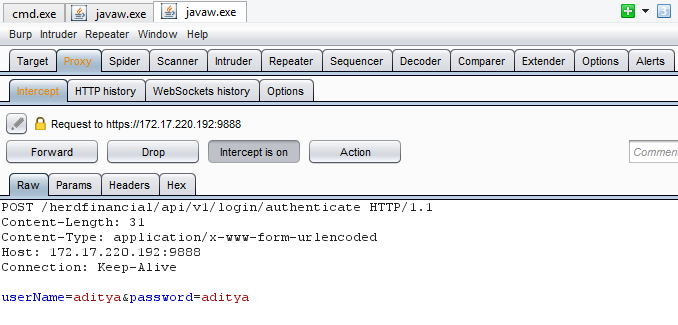
\includegraphics[width=14cm]{Imagens/burp.png} 
    \caption{Informação interceptada por proxy}
    Fonte: \citeonline{herd2016}
    \label{burp}
    \end{figure}

    O modelo proposto recomenda o uso do TLS para que as informações sejam transmitidas através de uma conexão que é totalmente criptografada e que a autenticidade tanto do servidor quanto do cliente sejam verificadas por meio de certificados digitais. 

    O código implementa uma conexão segura usando SSLSocket, que estabelece uma comunicação criptografada através de TLS. Isso garante que os dados transmitidos entre o cliente e o servidor sejam protegidos contra interceptação e manipulação, preservando a integridade e a confidencialidade das informações em trânsito.
    \\

    \begin{scriptsize}
    \estiloJava
    \begin{lstlisting}[caption={Conexão criptografada com SSLSocket}, label=lst:javacode]
    SSLSocketFactory socketFactory;
    SSLSocket socket;
    socketFactory = (SSLSocketFactory) SSLSocketFactory.getDefault();
    try {
        socket = (SSLSocket) socketFactory.createSocket(IP, Porta);
        System.out.println("Connected!");
    } catch (IOException e) {
        e.printStackTrace();
    }
    \end{lstlisting}
    \end{scriptsize}

    
    Por fim, nota-se que a aplicação não utiliza nenhuma forma de manter a integridade da mesma, o que permite a um atacante alterar transações ou até a própria aplicação. Dessa foram, o modelo recomenda a utilização de assinatura digital com algoritmos de criptografia assimétrica para garantir a procedência das informações e algoritmos de hash para garantir a integridade. 

    O código implementa uma assinatura digital usando o algoritmo ECDSA e verifica a integridade dos dados utilizando o hash criptográfico SHA-256. A assinatura digital garante que os dados ou transações não foram alterados desde que foram assinados, enquanto o hash criptográfico assegura que o conteúdo não foi modificado, protegendo assim a integridade e a autenticidade das informações.
    \\

    \begin{scriptsize}
    \estiloJava
    \begin{lstlisting}[caption={Assinatura digital com ECDSA e Hash criptográfico utilizando SHA-256}, label=lst:javacode]
    // Gerando uma assinatura digital
    byte[] message = "Texto plano";
    PrivateKey key = "Chave Privada";
    Signature s = Signature.getInstance("SHA256withECDSA");
    s.initSign(key);
    s.update(message);
    byte[] signature = s.sign();

    // Verificando uma assinatura digital
    byte[] message = "Texto plano";
    byte[] signature = "Assinatura";
    PublicKey key = "Chave Pública";
    Signature s = Signature.getInstance("SHA256withECDSA");
    s.initVerify(key);
    s.update(message);
    boolean valid = s.verify(signature);


    // Criptografia de Hash utilizando o algoritmo SHA-256
    byte[] message = "Texto plano";
    MessageDigest md = MessageDigest.getInstance("SHA-256");
    byte[] digest = md.digest(message);
    
    \end{lstlisting}
    \end{scriptsize}

    \section{Avaliação}

    A avaliação do modelo de segurança foi feita por meio da certificação PCI DSS, citada na seção \ref{pci} e desenvolvido pela \citeonline{pci2022}, com a verificação do cumprimento de 12 requisitos fundamentais exigidos pela organização. A conformidade com o PCI DSS não é apenas uma exigência das principais bandeiras de cartão de crédito, mas também uma medida crítica para minimizar riscos e fortalecer a confiança dos consumidores. Estes requisitos são projetados para cobrir todos os aspectos críticos da segurança da informação, desde a proteção da infraestrutura de rede até a implementação de políticas de segurança organizacional. 

    Na tabela \ref{tab:pci12} são mostrados os 12 requisitos exigidos pela certificação e marcados com ``X'' os quais o modelo proposto contempla. 

    \begin{table}[!htb]
    \centering
    \caption{12 requisitos do PCI DSS}
    \label{tab:pci12}
    \begin{tabular}{|l|c|}
    \hline
    \multicolumn{1}{|c|}{\textbf{Principais Requisitos do PCI DSS}}                                                                                                               & \textbf{Modelo} \\ \hline
    Instalar e manter controles de segurança de rede                                                                                                                     & X               \\ \hline
    \begin{tabular}[c]{@{}l@{}}Aplicar as configurações de segurança para todos os componentes de \\ sistema\end{tabular}                                                & X               \\ \hline
    Proteger os dados da conta armazenados                                                                                                                               & X               \\ \hline
    \begin{tabular}[c]{@{}l@{}}Proteger os dados do titular do cartão com criptografia forte durante\\ a transmissão em redes públicas abertas\end{tabular}              & X               \\ \hline
    Proteger todos os sistemas e redes de software malicioso                                                                                                             & X               \\ \hline
    Desenvolver e manter sistemas e software seguros                                                                                                                     & X               \\ \hline
    \begin{tabular}[c]{@{}l@{}}Restringir o acesso aos componentes de sistema e aos dados do titular\\ do cartão por necessidade de conhecimento do negócio\end{tabular} & X               \\ \hline
    Identificar usuários e autenticar o acesso aos componentes de sistema                                                                                                & X               \\ \hline
    Restringir o acesso físico aos dados do titular do cartão                                                                                                            &                 \\ \hline
    \begin{tabular}[c]{@{}l@{}}Registrar e monitorar todo o acesso aos componentes de sistema e \\ dados do titular do cartão\end{tabular}                               &                 \\ \hline
    Testar a segurança de sistemas e redes regularmente                                                                                                                  &                 \\ \hline
    Apoiar a segurança com políticas e programas organizacionais                                                                                           &                 \\ \hline
    \end{tabular}
    \end{table}

    \subsection{Análise de adequação}

    A seguir, é apresentada uma análise do modelo de requisitos de segurança para aplicações bancárias no Android em relação aos 12 requisitos fundamentais do PCI DSS, organizados em suas respectivas categorias. 

    \begin{enumerate}
        \item Construir e manter uma rede e sistemas seguros
            \begin{enumerate}
            \item \textbf{Instalar e manter controles de segurança de rede:} O modelo proposto não menciona explicitamente o uso de controles de monitoramento de rede, como firewalls ou IPS. Entretanto, ele restringe a interceptação de rede por meio do armazenamento dos certificados digitais confiáveis. 
            \item \textbf{Aplicar as configurações de segurança para todos os componentes de sistema:} O modelo sugere configurações de segurança para componentes do Android, como o uso de permissões rigorosas e validação de componentes, o que atende a este requisito.
            \end{enumerate}

        \item Proteger os dados da conta
            \begin{enumerate}
            \item \textbf{Proteger os dados da conta armazenados:} O modelo aborda a proteção dos dados armazenados com criptografia forte, como AES-256-CBC e SHA-256, o que cumpre este requisito.
            \item \textbf{Proteger os dados do titular do cartão com criptografia forte durante a transmissão em redes públicas abertas:} O uso de TLS 1.3 para criptografia de dados em trânsito, conforme recomendado no modelo, atende a este requisito.
            \end{enumerate}

        \item Manter um programa de gestão de vulnerabilidade
            \begin{enumerate}
            \item \textbf{Proteger todos os sistemas e redes de software malicioso:} O modelo menciona o uso de mecanismos de segurança da própria plataforma Android para proteção contra malwares, o que satisfaz este requisito. 
            \item \textbf{Desenvolver e manter sistemas e software seguros:} O modelo aborda a segurança durante o desenvolvimento de aplicações, o que é alinhado com este requisito. 
            \end{enumerate}

        \item Implementar medidas fortes de controle de acesso
            \begin{enumerate}
            \item \textbf{Restringir o acesso aos componentes de sistema e aos dados do titular do cartão por necessidade de conhecimento do negócio:} O modelo propõe a utilização de medidas de segurança nativas, como verificação e sanitização de intenções e uso de permissões, que são medidas adequadas para restringir o acesso com base na necessidade da plataforma; assim, contemplando este requisito. 
            \item \textbf{Identificar usuários e autenticar o acesso aos componentes de sistema:} A proposta de autenticação multifatorial (MFA) e autenticação de cada ação do usuário atende a este requisito.
            \item \textbf{Restringir o acesso físico aos dados do titular do cartão:} O modelo proposto  foca em controles de acesso digital e não aborda o controle de acesso físico. 
            \end{enumerate}

        \item Monitorar e testar as redes regularmente
            \begin{enumerate}
            \item \textbf{Registrar e monitorar todo o acesso aos componentes de sistema e dados do titular do cartão:} O modelo não contempla práticas de monitoramento e logging.
            \item \textbf{Testar a segurança de sistemas e redes regularmente:} O modelo não contempla recomendações de testes de segurança.
            \end{enumerate}

        \item Manter uma política de segurança da informação
            \begin{enumerate}
            \item \textbf{Apoiar a segurança da informação com políticas e programas organizacionais:} O modelo não menciona explicitamente a existência de políticas e programas organizacionais de segurança da informação.
            \end{enumerate}
    \end{enumerate}


    \subsection{Defesa do modelo}
    
    O modelo de segurança proposto cobre muitos dos aspectos fundamentais de segurança, como criptografia, autenticação, e controle de acesso, que são exigidos pelo PCI DSS. Em contraponto, algumas áreas, principalmente as relacionadas a infraestrutura e governança, não são contempladas, o que não garante conformidade total com a certificação PCI DSS. 

    Entretanto, como o resultado deste trabalho é um modelo de requisitos de segurança desenvolvido especificamente para aplicações bancárias no Android, a adequação do modelo ao seu propósito é demonstrada. O modelo foi elaborado para abordar os desafios únicos e as ameaças específicas enfrentadas por aplicações financeiras móveis, garantindo assim que as soluções propostas sejam diretamente aplicáveis e eficazes no contexto do Android.

    Portanto, afirmamos a adequação do modelo de requisitos de segurança proposto, pois ele fornece uma estrutura abrangente e direcionada para a proteção das aplicações bancárias no Android, considerando as necessidades específicas dessa plataforma e as expectativas do setor financeiro em termos de segurança e conformidade; chegando a conclusão que ele garante a segurança da informação.

    \section{Considerações finais do trabalho}
    O trabalho revelou diversas vulnerabilidades comuns em aplicações bancárias para Android, entre as principais ameaças identificadas estão os ataques de malware, falhas na autenticação, criptografia fraca e vulnerabilidades de rede. Os achados desta análise corroboram com o referencial teórico discutido anteriormente, especialmente com as diretrizes e recomendações da OWASP Mobile Top 10 descritas no tópico \ref{owasp} que engloba a maioria das ameaças citadas na literatura relacionada a segurança das aplicações bancárias. Dessa forma, fica evidente, tanto na literatura quanto nos resultados deste estudo, a importância dos requisitos de segurança bem definidos.

    Também nota-se que o resultado obtido neste estudo, isso é, o modelo de requisitos de segurança; está em consonância com as melhores práticas e recomendações encontradas na literatura sobre segurança em aplicações móveis, especialmente no contexto bancário. Os resultados deste estudo não apenas confirmam as melhores práticas recomendadas pelos artigos citados, encontrados na seção \ref{bancos}, mas também proporcionam uma definição, modelagem e avaliação de requisitos de segurança no cenário específico. 

    Com isso, a contribuição central deste estudo está na integração e na modelagem das práticas recomendadas encontradas na literatura em um modelo de segurança que destaca a relevância e a importância das medidas de segurança implementadas. Ao integrar e modelar informações de diversos artigos, conseguimos desenvolver um conjunto de práticas que pode servir como referência para a criação de futuras aplicações bancárias móveis seguras. O estudo de caso dos requisitos de segurança propostos mostrou-se eficaz na mitigação de vulnerabilidades, aprimorando significativamente a segurança da aplicação. O estudo de caso evidenciou como os requisitos de segurança modelados se comportam no cenário financeiro, demonstrando a importância de práticas de segurança bem estruturadas e contínuas para proteger aplicações bancárias móveis.

    Dessa forma, o modelo proposto nessa monografia têm implicações práticas significativas para desenvolvedores de aplicativos bancários, instituições financeiras e especialistas em cibersegurança. A implementação desses requisitos de segurança podem gerar sérios impactos positivos no desenvolvimento de aplicações bancárias no Android. Dentre elas o aumento da segurança das aplicações e da confiança dos clientes, com a implementação de medidas de segurança avançadas; a redução de riscos e custos, com a proteção da reputação da instituição financeira associado a diminuição dos riscos, violações de segurança e ataques cibernéticos; e melhores adaptações à regulamentações de segurança, com o auxílio para instituições financeiras a estar em conformidade com regulamentações rigorosas de proteção de dados. 
    
    Apesar dos resultados promissores esperados com a implementação do modelo de segurança para aplicações bancárias no Android, este estudo apresenta algumas limitações que devem ser consideradas. Primeiramente, a validação das medidas de segurança foi realizada em um ambiente controlado e teórico. Embora esse ambiente tenha permitido a avaliação detalhada de cada componente do modelo, ele não reproduz completamente as condições e desafios encontrados em ambientes de produção reais e práticos, onde fatores como a diversidade de dispositivos, versões do sistema operacional e comportamentos de usuários podem influenciar a eficácia das medidas de segurança implementadas.
    
    Além disso, a natureza dinâmica das ameaças à segurança cibernética implica que novas vulnerabilidades e métodos de ataque podem surgir continuamente. O modelo proposto, embora robusto, pode necessitar de atualizações e adaptações constantes para se manter eficaz contra novas formas de ataque. A rapidez com que essas ameaças evoluem pode superar a capacidade do modelo de responder em tempo hábil, especialmente se não houver um processo de monitoramento e atualização contínuo. Com isso, a sofisticação crescente dos ataques requer uma colaboração entre a indústria e a academia a fim de encontrar soluções inovadoras e uma abordagem proativa à segurança.

    Outro ponto a ser destacado é a especificação relacionada ao escopo das funcionalidades avaliadas. Este estudo focou principalmente em medidas de segurança diretamente relacionada as entendidas maiores ameaças encontradas em aplicações bancárias. No entanto, devem ser avaliadas todas as ameaças catalogadas e outras áreas da segurança também devem ser levadas em consideração durante a implementação de qualquer aplicação bancárias.